%%%%%%%%%%%%%%%%%%%%%%%%%%%%%%%%%%%%%%%%%%%%%%%%%
%%%%%%%%%%%%%%%%%%%%%%%%%%%%%%%%%%%%%%%%%%%%%%%%%

\chapter{Experimental Setup}
\label{chap:third}

%%%%%%%%%%%%%%%%%%%%%%%%%%%%%%%%%%%%%%%%%%%%%%%%%
%%%%%%%%%%%%%%%%%%%%%%%%%%%%%%%%%%%%%%%%%%%%%%%%%

%The same structure as before, including section, subsections and sub-subsections. Make sure that you follow the same conventions throughout, to avoid confusing the reader. Always remember to include a summary.

%%%%%%%%%%%%%%%%%%%%%%%%%%%%%%%%%%%%%%%%%%%%%%%%%
%%%%%%%%%%%%%%%%%%%%%%%%%%%%%%%%%%%%%%%%%%%%%%%%%
\section{Simulator}
A spatially discrete 2-dimensional grid world simulator has been developed and is used for the experimentation in order to accelerate computation \cite{sugawara2002swarming} and also because algorithm performance is sensitive to the amount of time taken to pickup item as well as the manoeuvring capabilities of the robots used \cite{ostergaard2001emergent}. The 2-dimensional grid world simulator allows for movement and pickup time to be standardized across all algorithms for effective comparison. Future studies could include these factors as part of algorithm performance, but are removed for simplification. Each robot fits into one grid block and each item takes up one grid block. Only one item or robot can occupy a grid block at a time thus creating collisions and congestion. Items can be picked up or can form obstacles that robots must navigate around.

The prioritized and non-prioritized sinks were placed next to each other, on a single side of the environment to more accurately represent the type of environment that the problem is most likely to be applied to e.g. in mine tunnels. The sink placement differs from the more common placement at the centre of the environment. The sinks were marked by light beacons that all robots can detect and navigate towards.

%Parameter
\section{Parameters}
\label{parameters}

	
For each class of environment, the following configurations were tested: The environment grid size, $S=50,100,200$ where $S$ is the width and length of the grid and the percentage $p$ of the grid covered by objects, with $p= 5\%$, $20\%$, $50\%$, $70\%$, $90\%$. The ratio of prioritized to non-prioritized items $r$, is varied, where $r=0$, $0.2$,$0.25$, $0.333$, $0.5$, $0.667$, $0.75$, $0.8$, $1$. Honey bee specific parameters were selected based on \cite{seeley2009wisdom} as 
$t_{max}=200$ timesteps, $f_{max}=100$ timesteps, $\phi=0.8$ and $\rho=0.1$.
%TODO: The idea is to add more robots foraging the prioritized items.
The following performance measures were used: the percentage of each item foraged over time, average time a robot spent in waiting state, and the entropy of robot movement. Due to space constraints, only the percentage, $\sigma$, of prioritized items foraged is presented. 

For all algorithms, robots were initially configured to forage either the prioritized item or the non-prioritized item with a ratio of $\tau=0$, $0.2$, $0.25$, $0.333$, $0.5$, $0.667$, $0.75$, $0.8$,$1$. Different numbers of robots, $c$, were used with $c=10, 30, 50, 70, 100$; $c$ is defined as the percentage of cells of the grid size $S$ that are occupied by robots.

\section{Performance Measures}
\label{thri:third:performancemeasures}

	\begin{itemize}
		\item	Amount gold items foraged over time
		\item	Amount waste items foraged over time
		\item	Average distance each robot moves
		\item	Average Time to forage an item for all robots
		\item	Average time to locate an item for all robots
		\item	Average time to return an item for all robots
		\item	Entropy of robot movement
	\end{itemize}
	
%%%%%%%%%%%%%%%%%%%%%%%%%%%%%%%%%%%%%%%%%%%%%%%%%

\section{Environment Types}
\label{thri:third:environmenttypes}

Four different classes of environments were used as follows:
\begin{enumerate}
\item Environments where items of each type are uniformly distributed (Fig \ref{fig:uniformenv}).
\item Clustered environments with clusters of item types generated by randomly relabelling items in clusters generated by Lumer-Faieta ant cemetery clustering \cite{lumer1994diversity} as either prioritized or non-prioritized items (Fig \ref{fig:clusterenv}).
\item Vein environments resembling the natural occurrence of gold \cite{frimmel2002recent} (Fig \ref{fig:veinenv}).
\item Gaussian environments where prioritized items are focused at the environment center. (Fig \ref{fig:gaussianenv}). %These environments are used to specifically examine how an algorithm can deal with moving past non-prioritized items to reach prioritized items. 
\end{enumerate} 

\vspace{-2em}
\begin{figure} [h]
        \centering
        \begin{subfigure}[b]{0.21\textwidth}
                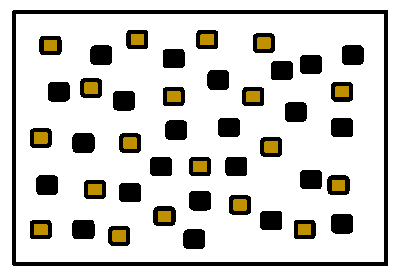
\includegraphics[width=\textwidth]{diagrams/uniformenv.pdf}
                \caption{Uniform}
                \label{fig:uniformenv}
        \end{subfigure}%
        \begin{subfigure}[b]{0.205\textwidth}
                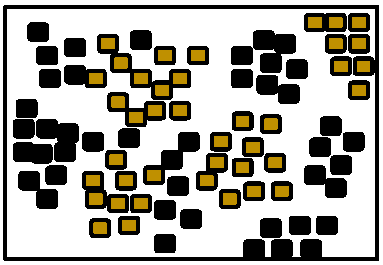
\includegraphics[width=\textwidth]{diagrams/clusterenv.pdf}
                \caption{Clustered}
                \label{fig:clusterenv}
        \end{subfigure}
        \begin{subfigure}[b]{0.2\textwidth}
                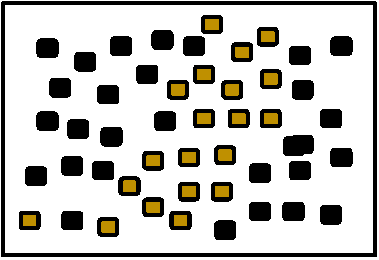
\includegraphics[width=\textwidth]{diagrams/veinenv.pdf}
                \caption{Vein}
                \label{fig:veinenv}
        \end{subfigure}  
        \begin{subfigure}[b]{0.2\textwidth}
                        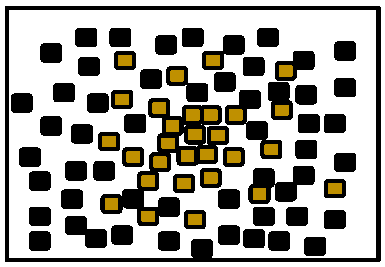
\includegraphics[width=\textwidth]{diagrams/gaussianenv}
                        \caption{Gaussian}
                        \label{fig:gaussianenv}
       \end{subfigure}
        \caption{Environment Classes}\label{fig:environments}
\end{figure}


%%%%%%%%%%%%%%%%%%%%%%%%%%%%%%%%%%%%%%%%%%%%%%%%%
%%%%%%%%%%%%%%%%%%%%%%%%%%%%%%%%%%%%%%%%%%%%%%%%%
\section{Summary}
\label{fourth:summary}

%%%%%%%%%%%%%%%%%%%%%%%%%%%%%%%%%%%%%%%%%%%%%%%%%
%%%%%%%%%%%%%%%%%%%%%%%%%%%%%%%%%%%%%%%%%%%%%%%%%